\documentclass[10pt,aspectratio=43,xcolor=x11names,t]{beamer}%aspectratio=169,


%\usepackage[space=false]{ctex}
\usepackage{fontspec,xunicode,xltxtra}
\usepackage{hyperref}	
\usepackage{booktabs}	
\usepackage{mathrsfs,amssymb,amsfonts,amsmath,bm}	%Math packages
\usepackage{dsfont}     %double line number
\usepackage{color}
\usepackage{xcolor}
\usepackage{graphicx,psfrag}
\usepackage{epsfig}
\usepackage{array, booktabs}
\usepackage{graphicx}
\usepackage{caption}
\usepackage{slashed}	%Dirac Operator
\usepackage{tikz}
	\usetikzlibrary{calc}
	\usetikzlibrary{decorations.markings}
	\usetikzlibrary{arrows}
\usepackage{extarrows}


\def\Re{\mathop{\mathcal{R}e}}
\def\Im{\mathop{\mathcal{I}m}}
\def\arrow{\tikz[scale=0.1,baseline=.1ex]{
	\draw[fill=black,rotate=-90] (-0.7,0)--(0,2)--(0.7,0);}
	}

\def\cross{\tikz[scale=0.1,baseline=.1ex]{
	\draw[thick,rotate=45] (-1,0)--(1,0);
	\draw[thick,rotate=45] (0,-1)--(0,1);}
	}

\newcommand*\dd{\mathop{}\!\mathrm{d}}
\newcommand*\ddd[1]{\mathop{}\!\mathrm{d^#1}}
\def\Re{\mathop{\mathcal{R}e}}					%Real part
\def\Im{\mathop{\mathcal{I}m}}					%imaginary part
\def\imp{\text{imp}}

\mode <presentation>
%\usetheme{Madrid}%% default Warsaw [secheader]
%\usetheme{Warsaw}%% tested by hxd
\usetheme{CambridgeUS}
\usecolortheme{beaver} %% changed by hxd, red style
\beamersetaveragebackground{black!10} % gray scale background

\setbeamercovered{transparent}
%\setbeamertemplate{navigation symbols}{}

\usefonttheme{professionalfonts}
\useinnertheme{circles}%{rectangles}
\setbeamertemplate{itemize item}{$\circledast$}% design the item bullet %\circledast  %\checkmark


\DeclareCaptionFont{blue}{\color{orange}}%LightSteelBlue3

\newcommand{\foo}{\color{blue}\makebox[0pt]{\textbullet}\hskip-0.5pt\vrule width 1pt\hspace{\labelsep}}%LightSteelBlue3

\hypersetup{pdfpagemode=FullScreen} % makes your presentation go automatically to full screen
%\setcounter{tocdepth}{1} % depth of table of contents

\defbeamertemplate{title page}{English}{ % English version of title page, use by \setbeamertemplate{title page}[Chinese/English]
	%\vbox{}
	\vfill
	\begin{center}
		\includegraphics[height=2.0cm]{BC-Eagle.svg}
		\vskip1em\par%
		\begin{beamercolorbox}[sep=8pt,center,shadow=true,rounded=true]{title}
			\usebeamerfont{title}\inserttitle\par%
			\ifx\insertsubtitle\@empty%
			\else%
				\vskip0.25em%
				{\usebeamerfont{subtitle}\usebeamercolor[fg]{subtitle}\insertsubtitle\par}%
			\fi%
		\end{beamercolorbox}%
		%\vskip1em\par
		%\begin{beamercolorbox}[sep=8pt,center]{author}
		%	\usebeamerfont{author}%\insertauthor
		%	{
		%	    \begin{tabular}{cc}
		%	    Respondant: &\insertauthor\\ %答辩人:
		%	    Supervisor: &\advisor %导\quad 师:
		%	    \end{tabular}
		%	}
		\end{beamercolorbox}
		\begin{beamercolorbox}[sep=6pt,center]{institute} %sep means separationb between beamercolorboxes
			\usebeamerfont{institute}\insertinstitute
		\end{beamercolorbox}
		\begin{beamercolorbox}[sep=6pt,center]{date}
			\usebeamerfont{date}\insertdate
		\end{beamercolorbox}\vskip0.5em
		%{\usebeamercolor[fg]{titlegraphic}\inserttitlegraphic\par}
	\end{center}
	\vfill
}

%\setbeamertemplate{section in toc}[ball,hideothersubsections]
%\setbeamertemplate{subsection in toc}[subsections numbered]


\setbeamertemplate{footline}{% change the ratio of each colorbox, cf. https://tex.stackexchange.com/questions/315580/how-to-adjust-width-of-footnotes-in-beamer-cambridgeus-theme/315587
	\leavevmode%
	\hbox{%
		\begin{beamercolorbox}[wd=.25\paperwidth,ht=2.25ex,dp=1ex,center]{author in head/foot}%
			\usebeamerfont{author in head/foot}\insertshortauthor\expandafter~~(\insertshortinstitute)
		\end{beamercolorbox}%
		\begin{beamercolorbox}[wd=.45\paperwidth,ht=2.25ex,dp=1ex,center]{title in head/foot}%
			\usebeamerfont{title in head/foot}\insertshorttitle
		\end{beamercolorbox}%
		\begin{beamercolorbox}[wd=.3\paperwidth,ht=2.25ex,dp=1ex,right]{date in head/foot}%
			\usebeamerfont{date in head/foot}\insertshortdate{}\hspace*{2em}
			\insertframenumber{} / \inserttotalframenumber\hspace*{2ex} 
		\end{beamercolorbox}
	}%
	\vskip0pt%
}

%%%%%%%%% set environments like block's color %%%%%%%%%%%
	\setbeamercolor{block title}{use=structure,fg=structure.fg,bg=structure.fg!20!bg}
	\setbeamercolor{block body}{parent=normal text,use=block title,bg=block title.bg!50!bg}

	\setbeamercolor{block title example}{use=example text,fg=example text.fg,bg=example text.fg!20!bg}
	\setbeamercolor{block body example}{parent=normal text,use=block title example,bg=block title example.bg!50!bg}

	\newenvironment<>{redblock}[1]{%
		\setbeamercolor{block title}{fg=white,bg=red!70!pink}%
		\begin{block}#2{#1}}{\end{block}
	}
	\newenvironment<>{greenblock}[1]{%
		\setbeamercolor{block title}{fg=white,bg=green!70!blue}%
		\begin{block}#2{#1}}{\end{block}
	}

	\addtobeamertemplate{proof begin}{%
		\setbeamercolor{block title}{fg=black,bg=red!50!white}
		\setbeamercolor{block body}{fg=red, bg=red!30!white}
	}{}

	\BeforeBeginEnvironment{theorem}{
		\setbeamercolor{block title}{fg=black,bg=orange!50!white}
		\setbeamercolor{block body}{fg=orange, bg=orange!30!white}
	}
	\AfterEndEnvironment{theorem}{
		\setbeamercolor{block title}{use=structure,fg=structure.fg,bg=structure.fg!20!bg}
		\setbeamercolor{block body}{parent=normal text,use=block title,bg=block title.bg!50!bg, fg=black}
	}

\begin{document}

\title[Haldane's Conjecture]{Nonlinear Field Theory of Large-Spin $1$d\\Heisenberg Antiferromagnets}
\subtitle{NL$\sigma$ Model, Semiclassical Soliton Quantization, and Mass Gap Conjecture}
\author[Xiaodong Hu]{F. D. M. Haldane\inst{1} \and Xiaodong Hu\inst{2}}
%\def\advisor{Prof. Guo-Zhu Liu$^{1}$\quad Prof. Ying-Hai Wu$^2$}
\institute[BC]{\inst{1} Princeton University \and \inst{2} Boston College}



\date{\color{red}\textit{Phys. Rev. Lett.} \textbf{50}, 1153 (1983)}

%\begin{minipage}{6in}
%\centering
%\raisebox{-0.5\height}{\includegraphics[width=1in]{Princeton.pdf}}
%\hspace*{.2in}
%\raisebox{-0.5\height}{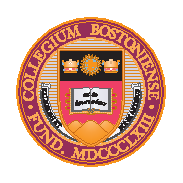
\includegraphics[width=0.5in]{BC-color.eps}}
%\end{minipage}
\titlegraphic{\includegraphics[height=0.5in]{Princeton.pdf}\hspace{0.3in}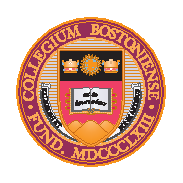
\includegraphics[height=0.5in]{BC-color.eps}}

\begin{frame}%[plain] % without section heads
	\titlepage
\end{frame}


\AtBeginSection[]{% add a frame of current position before every section
	\frame{
		\setcounter{tocdepth}{2}
		\frametitle{Contents}
		\tableofcontents[
			currentsection
		]
	}
}

\begin{frame}
	\frametitle{Contents}
	\tableofcontents
\end{frame}

%%%%%%%%%%%%%%%%%%%%%%%%%%%%%%%%%%%%%%%%%%%%%%%%%%%%%%%%%%%%%%%%%%%%%%%%%%%%%%%

\section{Introduction}
	\subsection{Previous Work}
		\begin{frame}\frametitle{N\'{e}el Order and Spin Waves in Classical AFM}
			\begin{columns}
				\begin{column}{0.5\textwidth}
					\textbf{\color{red}Classically}, isotropic \textbf{antiferromagnetic} Heisenberg model
					\begin{equation*}
						H=J\sum_n\bm{S}_n\cdot\bm{S}_{n+1}
					\end{equation*}
					in $d=1$ has
					\begin{itemize}
						\item A doubly degenerate ground state with anti-parallel alignment (\textbf{\color{red}long-range N\'{e}el order}).
						\item A low-energy \textbf{\color{red}gapless excitation} of spin wave ({\scriptsize Halperin\&Hohenberg, \textit{Phys. Rev.}, \textbf{188}, 898 (1969)})
						\begin{equation*}
							\omega_k=\omega\sin ka,\quad \omega\equiv 2JS
						\end{equation*}
					\end{itemize}
				\end{column}
				\pause
				\begin{column}{0.5\textwidth}
					\begin{block}{Holstein-Primakoff Transformation}
						Representing the $\mathfrak{su}(2)$ operator with bosonic creation and annihilation operators ($n_b\equiv b^\dagger b$)
						\begin{equation*}
							\begin{cases}
								S^z=S-n_b\\
								S^+=\bigg(\sqrt{2S-n_b}\bigg)b\\
								S^-=b^\dagger\bigg(\sqrt{2S-n_b}\bigg)
							\end{cases}
						\end{equation*}
						where $[b,b^\dagger]\equiv1$, and expanding in the order of $1/S$.
					\end{block}
				\end{column}
			\end{columns}
		\end{frame}

	\subsection{Question We Address}

		\begin{frame}\frametitle{Will These Two Properties Hold for Full Quantum Heisenberg Model?}
			\pause
			\begin{greenblock}{Mermin-Wagner Theorem}
				\begin{itemize}
					\item The is NO spontaneous symmetry breaking for Heisenberg models in dimension $d=1$. 
					\item Quantum fluctuation will destroy the long-range order.
				\end{itemize}
			\end{greenblock}
			So both of them cannot survive.
			\only<3->{
				\begin{itemize}
					\item \textbf{The ground state cannot be SYB ordered}.
					\item \textbf{The spin-wave description of elementary excitation is not enough}.
				\end{itemize}
			}
			\only<4>{
			\begin{block}{Know Result}
				\textbf{\color{red}Spin-1/2} antiferromagnetic Heisenberg model is exactly solvable!
				\begin{itemize}
					\item The ground state is found by Bethe ansatz ({\scriptsize Bethe, \textit{Zeitschrift für Physik}, \textbf{71}.3-4 (1931)}).
					\item The \textbf{\color{red}gapless} excitation is obtained by studying of $d=1$ delta-repulsion bosonic systems ({\scriptsize Yang\&Yang, J. Math. Phys., \textbf{10}.7 (1969)}).
				\end{itemize}
			\end{block}
			}
		\end{frame}
		\begin{frame}[c]
			\begin{redblock}{The Question We Adress}
				\begin{itemize}
					\item What is the ground state for $S=1$ or other larger spin-magnitude antiferromagnetic Heisenberg model?
					\item What is the correct low-energy effective theory of antiferromagnetic Heisenberg model?
					\item Will the \textbf{gapless excitation} still be true for $S=1$ or other larger spin magnitudes? 
				\end{itemize}
			\end{redblock}
		\end{frame}
		
\section{Low-energy Effective Field Theory of AFM}
	\subsection{Angle-variable Representation}
		\begin{frame}\frametitle{Classical Equations of Motion}
			Parameterizing each spin of the lattice on the Bloch sphere 
			\begin{equation*}
				\bm{S}_n=(-1)^n(\sin\theta_n\cos\varphi_n,\sin\theta_n\sin\varphi_n,\cos\theta_n),
			\end{equation*}
			then the classical equation of motion reads ($\omega\equiv 2JS$)
			\begin{block}{Classical EOM}
				\begin{align*}
					\dot{\theta}_n&=-\dfrac{\omega}{2}(-1)^n\sum_{\lambda=\pm}\sin\theta_{n\pm\lambda}\sin(\varphi_{n\pm\lambda}-\varphi_n),\\
					\dot{\varphi}_n&=-\dfrac{\omega}{2}(-1)^n\sum_{\lambda=\pm}\big(\cos\theta_{n\pm\lambda}-\cot\theta_n\sin\theta_{n\pm\lambda}\cos(\varphi_{n\pm\lambda}-\varphi_n)\bigg).
				\end{align*}
			\end{block}
			if we assign the canonical conjugate pair with the Poisson-backect
			\begin{equation*}
				\color{red}\{\varphi_n,S_{n'}^z\}\equiv\delta_{nn'}.
			\end{equation*}
		\end{frame}
		
	\subsection{Semi-classical Approximation}
		\begin{frame}\frametitle{Low-energy Gradient Expansion}
			\begin{itemize}
				\item We focus on the physics in long-wavelength (low-energy) regime $(a\ll1)$, so all field operators should vary \textbf{slowly} with lattice.
				\item To keep all nonlinear effects, the fluctuation of \textbf{both} branches of low-energy spin wave mods ($k=0$ and $k=\pi$) should be taken into account. 
			\end{itemize}
			\pause
			So we write
			\begin{equation*}
				\theta_n=\theta(x)+a(-1)^n\alpha(x),\quad \varphi_n\equiv\varphi(x)+a(-1)^n\beta(x).
			\end{equation*}
			for $x=na$ and expand the EOM with spatial gradient up to quadratic order.
			\only<3>{
			\begin{greenblock}{{\color{red}Low-energy} Classical EOM}
				\begin{align*}
					\dot{\theta}(x)&=\omega a\beta\sin\theta,&\dot{\alpha}(x)\sin\theta&=-\omega a\bigg[\nabla\left(\sin^2\theta\cdot\nabla\varphi\right)+\sin2\theta\cdot \alpha\beta\bigg],\\
					\dot{\varphi}(x)&=-\dfrac{\omega a}{\sin\theta}\alpha,&\dot{\beta}(x)\sin\theta&=\dfrac{\omega a}{2}(\nabla\theta)^2-\dfrac{\omega a}{4}\sin2\theta\bigg[(\nabla\varphi)^2-\left(\dfrac{2 \alpha}{\sin\theta}\right)^2+4\beta^2\bigg].
				\end{align*}
			\end{greenblock}}
		\end{frame}
		\begin{frame}\frametitle{Recognizing Conjugate Variables}
			\begin{greenblock}{{\color{red}Low-energy} Classical EOM}
				\begin{align*}
					\dot{\theta}(x)&=\omega a\beta\sin\theta,&\dot{\alpha}(x)\sin\theta&=-\omega a\bigg[\nabla\left(\sin^2\theta\cdot\nabla\varphi\right)+\sin2\theta\cdot \alpha\beta\bigg],\\
					\dot{\varphi}(x)&=-\dfrac{\omega a}{\sin\theta}\alpha,&\dot{\beta}(x)\sin\theta&=\dfrac{\omega a}{2}(\nabla\theta)^2-\dfrac{\omega a}{4}\sin2\theta\bigg[(\nabla\varphi)^2-\left(\dfrac{2 \alpha}{\sin\theta}\right)^2+4\beta^2\bigg].
				\end{align*}
			\end{greenblock}
			The low-energy EOM enlighten us to define the conjugate variables ($g\equiv2/S$)
			\begin{equation*}
				L(x)\equiv-2g^{-1}\alpha\sin\theta,\quad \Pi_\theta(x)\equiv2g^{-1}\beta\sin\theta,
			\end{equation*}
			and assign the Poisson bracket for them\only<2>{\footnote{\textbf{\color{red}Given a Hamiltonian, the EOM cannot be uniquely defined unless all conjugate variables are recognized!}}}
			\begin{equation*}
				\{\theta(x),\Pi_\theta(x')\}=\{\varphi(x),L(x')\}=\delta(x-x').
			\end{equation*}
		\end{frame}
		
	\subsection{Non-linear Sigma Model}
		\begin{frame}\frametitle{Effective Lagrangian}
			Then the above four nonlinear EOM can be derived from
			\begin{block}{Effective Hamiltonian}
				\begin{equation*}
					H=\dfrac{\omega a}{2}\int\dd x\bigg\{g\left(\Pi_\theta^2+\dfrac{L^2}{\sin^2\theta}\right)+\dfrac{1}{g}\bigg[(\nabla\theta)^2+(\nabla\varphi)^2\sin^2\theta\bigg]\bigg\}.
				\end{equation*}
			\end{block}
			\only<2>{
			And the corresponding Lagrangian density has a extreme neat form in terms of the \textbf{unit} vector $\bm{n}\equiv(\sin\theta\cos\varphi,\sin\theta\sin\varphi,\cos\theta)$
			\begin{redblock}{Effecitve Lagrangian}
				\begin{equation*}
					\mathcal{L}=\dfrac{1}{2g}\left[\dfrac{1}{c}(\partial_t\bm{n})^2-c(\nabla\bm{n})^2\right].
				\end{equation*}
			\end{redblock}
			where $c\equiv\omega a$. This is nothing but \textbf{\color{red} $O(3)$ Nonlinear $\sigma$-Model}.}

		\end{frame}

\section{Haldane's Conjecture}
	\subsection{Topological Soliton Solution}
		\begin{frame}\frametitle{The Fate of Vacua}
			Previous work:
			\begin{itemize}
				\item In the aspect of CMP, \textbf{the nonlinear EOM of NL$\sigma$M support the existence of topological soliton solutions}\\
				({\scriptsize Skyrme \textit{Proc. Roy. Soc. London A} \textbf{260} (1961); Belavin\&Polyakov, \textit{JEPT Lett.} \textbf{22}, 10 (1961)}).
				\item In the aspect of HEP, \textbf{different topological sectors of vacuum will tunnel to each other and result in the ``decay of vacua''}.\\
				({\scriptsize Berlavin\&Polyakov et al. \textit{Phys. Lett. B}, \textbf{59}, 1 (1975)})
			\end{itemize}
			\only<2>{
			\hfill\\[1em]
			Indication on our case:
			\begin{block}{The Fate of False Ground State}
				\begin{itemize}
					\item The \textbf{trivial} ordered ground state (spin wave) with gapless excitation will be unstable under the nonlinear effects --- proliferation of solitons. In such case the \textbf{large-$S$ limit} is suggested to be \textbf{\color{red}{gapped}}.
					\item We CANNOT rule out the possibility of other \textbf{nontrivial} stable phase with \textbf{\color{red}gapless} excitations.
				\end{itemize}
			\end{block}
			}
		\end{frame}
		\begin{frame}\frametitle{Contradiction?}
			\begin{block}{The Fate of False Ground State}
				\begin{itemize}
					\item The \textbf{trivial} ordered ground state (spin wave) with gapless excitation will be unstable under the nonlinear effects --- proliferation of solitons. In such case the \textbf{large-$S$ limit} is suggested to be \textbf{\color{red}{gapped}}.
					\item We CANNOT rule out the possibility of other \textbf{nontrivial} stable phase with \textbf{\color{red}gapless} excitations.
				\end{itemize}
			\end{block}
			\vspace{1em}
			\begin{figure}[!htp]
				\centering
				\includegraphics[scale=0.6]{RG.pdf}
			\end{figure}
			\only<2>{
			\begin{center}
				\vspace*{1em}
				RG analysis is necessary!
			\end{center}
			}
		\end{frame}
		
		\begin{frame}\frametitle{What's The Connection of Elementary Excitation with the Spin Magnitudes?}
			\begin{block}{RG of NL$\sigma$M}
				The $\beta$ function for coupling constant $g$ is obtained by $(2+\varepsilon)$-dimension expansion ({\scriptsize Brézin\&Zinn-Justin, \textit{PRL.}, \textbf{36}, 691 (1976); Polyakov, \textit{Phys. Lett. B}, \textbf{59}.1 (1975)})
				\begin{equation*}
					\beta(g)\equiv\dfrac{\dd g}{\dd\ln a}=\dfrac{g^2}{2\pi}+\dfrac{g^3}{(2\pi)^2}+\cdots\implies\text{Asymptotic Freedom}
				\end{equation*}
				where $a$ is the ultraviolate cutoff. 
			\end{block}
			Since the physical correlation length remains invariant under RG procedure $\beta(\xi)=0$, we can connect the correlation length on both sides. Particularly, in the \textbf{small-$S$ (strong-coupling) limit}
			\begin{equation*}
				\text{gap}^{-1}\simeq\color{red}\xi= ae^{\pi S}.
			\end{equation*}
		\end{frame}
		
\section{Summary}
	\subsection{Haldane's Conjecture}
		\begin{frame}\frametitle{Haldane's Conjecture}
			Let me summarizes our result:
			\begin{itemize}
				\item We obtain the low-energy effective field theory of $d=1$ antiferromagnetic Heisenberg model.
				\item We study the possible influence brought by the topological soliton solution.
				\item We try to connect the behavior of elementary excitation in the large-$S$ regime and small-$S$ regime, getting the result
			\end{itemize}
			\begin{center}
				\begin{tabular}{c|c|c|c}
					\hline
					& Small-$S$  & & Large-$S$\\
					\hline
					Half-Integer & Gapless & $\Longleftrightarrow$ & \\
					\hline
					Integer & & $\Longleftrightarrow$ & Gapped (possible)\\
					\hline
				\end{tabular}
			\end{center}
			\pause
			\begin{redblock}{Haldane's Conjecture}
				\begin{itemize}
					\item Half-integer spin antiferromagnetic Heisenberg models in $d=1$ is \textbf{gappless}.
					\item Integer spin antiferromagnetic Heisenberg models in $d=1$ is \textbf{gapped}.
				\end{itemize}
			\end{redblock}
		\end{frame}

	\subsection{Acknowledgement}
		\begin{frame}[c] % center the page
			\begin{center}
				{\fontsize{50}{60}\selectfont Thanks!}
			\end{center}
		\end{frame}





%%%%%%%%%%%%%%%%%%%%%%%%%%%%%%%%%%%%%%%%%%%%%%%%%%%%%%%%%%%%%%%%%%%%%%%%%%%%%%%
\iffalse
\section{Kondo Effect}
	\subsection{Experimental Review}
		\begin{frame}[t]\frametitle{Resistance Minimum}

		\end{frame}
		\begin{frame}[t]\frametitle{How to Understand This?}
			\begin{itemize}
				\item We know that for usual impurities like defects, conductivity (relaxation time) is not temperature-dependent.
				\item Even if we inlcude the contribution of electon-phonon scattering, Boltzmann equation still tells us that resistivity \emph{drops} in the manner of $\rho\sim\dfrac{1}{\tau}\propto T^5$ at low temperature region.
				\item It happens only for {\color{blue}magnetic impurities} (Here is Fe) $\implies$ There must be some microscopic mechanism that magnetism start to play a role at low temperature.
			\end{itemize}
			\pause
			\begin{block}{Anderson Model (Anderson \textit{Phys. Rev.} \textbf{124}, 41(1961))}
				\begin{equation*}
					H=\sum_{k \sigma}\varepsilon_kc_{k\sigma}^\dagger c_{k\sigma}+\sum_{\sigma}\varepsilon_d d_{\sigma}^\dagger d_{\sigma}+{\color{red}Un_{d\uparrow}n_{d\downarrow}}+\sum_{k\sigma}V_k\big(c_{k\sigma}^\dagger d_{\sigma}+h.c.\big)
				\end{equation*}
				\centering Strong Correlation of impurities is necessary!
			\end{block}	
		\end{frame}

	\subsection{Anderson Model}
		\begin{frame}[t]\frametitle{Mean-Field Solution (Hartree-Fock)}
			MF treatment of Hubbard term
			\begin{equation*}
				H_d=\sum_{\sigma}\varepsilon_d d_\sigma^\dagger d_\sigma+U(\langle n_{d\downarrow}\rangle n_{d\uparrow}+\langle n_{d\uparrow}\rangle n_{d\downarrow}-\langle n_{d\uparrow}\rangle \langle n_{d\downarrow}\rangle )
			\end{equation*}
			\pause
			Treating both $V_k\equiv V$ and the host DOS $\rho(\varepsilon)=\rho_0$ as constants, and denoting $\Delta\equiv\pi V^2\rho(\varepsilon)$, then after integrating out the itinerate electrons we obtain the Green function for impurities
			\begin{equation*}
				G_{d\sigma}(\omega)=\dfrac{1}{\omega-E_{d\sigma}+i\Delta},\quad\text{where }E_{d\sigma}=\varepsilon_d+\rho_0 |V|^2\ln\left|\dfrac{\varepsilon_d-D}{\varepsilon_d+D}\right|+U \langle n_{d\bar\sigma} \rangle
			\end{equation*}
			So DOS and the occupation number are
			\begin{align*}
				\rho_{d\sigma}(\varepsilon)&\equiv-\dfrac{1}{\pi}\mathcal{I}m G_{d\sigma}=\dfrac{1}{\pi}\dfrac{\Delta}{(\varepsilon-E_{d\sigma})^2+\Delta^2},\\
				\langle n_{d\sigma}\rangle &\equiv\int_{-\infty}^\mu\dd \varepsilon\, n_F(\varepsilon)\rho_{d\sigma}(\varepsilon)=\dfrac{1}{2}-\arctan\dfrac{E_{d\sigma}-\mu}{\Delta},
			\end{align*}
		\end{frame}
		\begin{frame}[t]\frametitle{Success: Magnetic Impurities}
			\begin{columns}
				\begin{column}{0.4\textwidth}
					Anderson obtain a $T=0$ phase diagram for proof of local moments for impurities
					\begin{equation*}
						\langle S_z \rangle \sim \langle n_{d\uparrow}-n_{d\downarrow} \rangle\simeq\dfrac{1}{\pi}\arctan\dfrac{2\langle S_z \rangle U}{\Delta}
					\end{equation*}
					Only when $\dfrac{U}{\pi\Delta}>1$ will the moment exists.
					\pause
					\begin{redblock}{Magnetic Phase}
						Impurities are magnetic only {\color{blue}at large U limit} with small DOS of itinerate eletrons.
					\end{redblock}
				\end{column}
				\begin{column}{0.4\textwidth}

				\end{column}
			\end{columns}
		\end{frame}
		\begin{frame}[t]\frametitle{Flaws of Mean-Field Treatment}
			\begin{itemize}
				\item {\color{blue}We obtain a phase transition even at a finite system}. 
					\begin{itemize}
					 	\item Since $\langle S_z \rangle\neq0$, this is a ususal symmetry-breaking phase transition (rather than quantum phase transition characterized by the long-range behavior of Green functions). However, by definition, in Ginzberg-Landau theory the oder parameter become nonzero only when we goes to thermodynamics limit.
					 \end{itemize}
				\item {\color{blue}The correlation time scale is much shorter than the lifetime of Impurity State}
					\begin{itemize}
						\item Correlation time scale is proportional to $1/U$ while from the imaginary part of Green function the lifetime of this state is proportional to $1/\Delta$. Existence of magnetic moment require $U\gg\Delta$, so $1/U\ll1/\Delta$ is again unacceptable.
					\end{itemize}
				\item {\color{blue}The state that minimize the Hartree-Fock energy is NOT the real ground state.}
					\begin{itemize}
						\item In strongly-correlated system like Heisenberg model for antiferromagnetic case, the quantum fluctuation is extremely important that single particle picture will totally breakdown!
					\end{itemize}
			\end{itemize}
		\end{frame}
	\subsection{Low-energy Effective Hamiltonian}		
		\begin{frame}\frametitle{Low Energy Effective Hamiltonian}
			Let us focus on single impurity.
			\begin{itemize}
				\item Large U limit and half-filling condition highly suppressed the mobility of impurity eletrons.
				% Or more precisely, doubly occupied or empty states are energetic forbidden while (quantum) superexchange mechanism still work here.
				\item So the charge degree of freedom is quenched while {\color{blue}superexchange mechanism} (Anderson \textit{Phys. Rev.} \textbf{79}, 350 (1950)) still works for spin degree of freedom. Therefore, the low-energy effective Hamiltonian must be spin Hamiltonian for impurity electrons.  
			\end{itemize}
			\pause
			To realize the above physical confinement, we should separate the entire many-body Hilbert space as orthogonal subspaces with doubly occupied $|\psi_2\rangle$, singly occupied $|\psi_1\rangle$, or empty states $|\psi_0\rangle$ and {\color{blue}project out the unphysical first and last one}.
		\end{frame}
		\begin{frame}\frametitle{Schrieffer-Wolff Transformation {\scriptsize(Schrieffer\&Wolff \textit{Phys. Rev.} \textbf{149}, 491 (1966))}}
			
			With projection operator $P_2=n_{d\uparrow}n_{d\downarrow}, P_1=n_{d\uparrow}(1-n_{d\downarrow})+n_{d\downarrow}(1-n_{d\uparrow})$, and $P_0=\mathds{1}-P_1-P_2$ we have explicitly
			\begin{columns}
				\begin{column}{0.5\textwidth}
					\begin{align*}
						H_{00}&\equiv P_0HP_0\\
						&=\sum_{k \sigma}\varepsilon_{k}c_{k\sigma}^\dagger c_{k\sigma},\\
						H_{11}&\equiv P_1HP_1\\
						&=\sum_{k \sigma}\varepsilon_{k}c_{k\sigma}^\dagger c_{k\sigma}+\varepsilon_d,\\
						H_{22}&\equiv P_2HP_2\\
						&=\sum_{k \sigma}\varepsilon_{k}c_{k\sigma}^\dagger c_{k\sigma}+2 \varepsilon_d+U,
					\end{align*}
				\end{column}
				\begin{column}{0.5\textwidth}
					\begin{align*}
						H_{01}&\equiv P_0HP_1\\
						&=\sum_{k\sigma}V_kc_{k\sigma}^\dagger d_\sigma n_{d\sigma}(1-n_{d\bar{\sigma}})\\
						H_{12}&\equiv P_1HP_2\\
						&=\sum_{k\sigma}V_kc_{k\sigma}^\dagger d_\sigma n_{d\sigma}n_{d\bar{\sigma}}\\
						H_{02}&\equiv P_0HP_2=0.
					\end{align*}
				\end{column}
			\end{columns}
		\end{frame}
		\begin{frame}\frametitle{Schrieffer-Wolff Transformation {\scriptsize(Schrieffer\&Wolff \textit{Phys. Rev.} \textbf{149}, 491 (1966))}}
			\begin{block}{Schrieffer-Wolff Transformation}
				Schrieffer-Wolff transformation is a canonical transformation diagnalizing the \emph{many-body Hamiltonian} with distinct number of occupations
				\begin{align*}
					\widetilde{H}\equiv e^{S}He^{-S}&=H+[S,H]+\dfrac{1}{2!}[S,[S,H]]+\cdots\nonumber\\
					&=H_0+V+[S,H_0]+[S,V]+\dfrac{1}{2!}[S,[S,H_0+V]]+\cdots
				\end{align*}
				such that $V+[S,H_0]\equiv0.$ So up to the second order we are left with
				\begin{equation*}
					\widetilde{H}^{(2)}=H_0+[S,V]+\dfrac{1}{2}[S,[S,H_0]]=H_0+\dfrac{1}{2}[S,H_0].
				\end{equation*}
			\end{block}
			\pause
			{\color{red}This is also some renormalization procedure for gapped system!}
		\end{frame}
		\begin{frame}\frametitle{Schrieffer-Wolff Transformation}
			 After lenthy calculation of commutators, up to some constant, we obtain the second order effective Hamiltonian
			 \begin{equation*}
			 	H_{\text{eff}}^{(2)}=\sum_{k \sigma}\varepsilon_k c_{k \sigma}^\dagger c_{k \sigma}+\sum_{kk' \sigma\sigma'}V_k^*V_{k'}\left(\dfrac{d_\sigma^\dagger d_{\sigma'}}{\varepsilon_d- \varepsilon_{k'}}c_{k \sigma}c_{k'\sigma'}^\dagger+\dfrac{d_\sigma d_{\sigma'}^\dagger}{U+\varepsilon_d- \varepsilon_{k'}}c_{k \sigma}^\dagger c_{k'\sigma'}\right).
			 \end{equation*}
			 Introducing the second quantized spin operator $\bm{S}_{kk'}\equiv\sum_{\alpha \beta}c_{k \alpha}^\dagger\dfrac{\bm{\sigma}_{\alpha \beta}}{2}c_{k \beta}$ and $\bm{S}_d\equiv\sum_{\mu\nu}d_\mu^\dagger\dfrac{\bm{\sigma}_{\mu\nu}}{2}d_{\nu},$ we finally get the Low-energy Effective Spin Hamiltonian
			 \begin{greenblock}{s-d Hamiltonian}
			 	\begin{equation*}
			 		H_{sd}=\sum_{k \sigma}\varepsilon_k c_{k \sigma}^\dagger c_{k \sigma}+\sum_{kk'}J\bm{S}_{kk'}\cdot\bm{S}_d,
			 	\end{equation*}
			 \end{greenblock}
		\end{frame}
	\subsection{Warmup: Relaxation time from Spin Scattering}
		\begin{frame}\frametitle{Warmup: Interactive Green Function}
			Functional derivative of partition function with auxilliary fields tells us
			\begin{align*}
				%\begin{tikzpicture}[> = latex,decoration = {markings,mark=at position 0.6 with {\arrow[very thick]{latex}}}]
				%	\draw[double,postaction={decorate},thick] (0,0)--(2,0);
				%\end{tikzpicture}
				\begin{tikzpicture}[scale=0.8,baseline]
					\draw[double,thick] (0,0)-- (2,0);
					\node at (1,0) {\arrow};
				\end{tikzpicture}
				&=
				\begin{tikzpicture}[scale=0.8,baseline]
					\draw[thick] (0,0)-- (2,0);
					\node at (1,0) {\arrow};
				\end{tikzpicture}
				+
				\left(
				\begin{tikzpicture}[scale=0.8]
					\draw[thick] (0,0)--(2,0);
					\draw[thick,dashed] (1,1)--(1,0);
					\node at (1,1) {\cross};
				\end{tikzpicture}
				+
				\begin{tikzpicture}[scale=0.8]
					\draw[thick] (0,0)--(3,0);
					\draw[thick,dashed] (1,1)--(1,0);
					\draw[thick,dashed] (2,1)--(2,0);
					\node at (1,1) {\cross};
					\node at (2,1) {\cross};
				\end{tikzpicture}
				+\cdots\right)\\
				&+
				\left(
				\begin{tikzpicture}[scale=0.8]
					\draw[thick] (0,0)--(2,0);
					\draw[thick,dashed] (0.6,0)--(1,1);
					\draw[thick,dashed] (1.4,0)--(1,1);
					\node at (1,1) {\cross};
				\end{tikzpicture}
				+
				\begin{tikzpicture}[scale=0.8]
					\draw[thick] (0,0)--(3,0);
					\draw[thick,dashed] (0.6,0)--(1,1);
					\draw[thick,dashed] (1.4,0)--(1,1);
					\draw[thick,dashed] (1.6,0)--(2,1);
					\draw[thick,dashed] (2.4,0)--(2,1);
					\node at (1,1) {\cross};
					\node at (2,1) {\cross};
				\end{tikzpicture}
				+
				\begin{tikzpicture}[scale=0.8]
					\draw[thick] (0,0)--(4,0);
					\draw[thick,dashed] (0.6,0)--(1,1);
					\draw[thick,dashed] (1.4,0)--(1,1);
					\draw[thick,dashed] (1.6,0)--(2,1);
					\draw[thick,dashed] (2.4,0)--(2,1);
					\draw[thick,dashed] (2.6,0)--(3,1);
					\draw[thick,dashed] (3.4,0)--(3,1);
					\node at (1,1) {\cross};
					\node at (2,1) {\cross};
					\node at (3,1) {\cross};
				\end{tikzpicture}
				\right)\\
				&+\left(\begin{tikzpicture}[scale=0.8]
					\draw[thick] (0,0)--(2.8,0);
					\draw[thick,dashed] (0.6,0)--(1,1);
					\draw[thick,dashed] (1.4,0)--(1,1);
					\draw[thick,dashed] (2,0)--(2,1);
					\node at (1,1) {\cross};
					\node at (2,1) {\cross};
				\end{tikzpicture}
				+
				\begin{tikzpicture}[scale=0.8]
					\draw[thick] (0.2,0)--(3,0);
					\draw[thick,dashed] (1.6,0)--(2,1);
					\draw[thick,dashed] (2.4,0)--(2,1);
					\draw[thick,dashed] (1,0)--(1,1);
					\node at (1,1) {\cross};
					\node at (2,1) {\cross};
				\end{tikzpicture}+\cdots\right)+\cdots,
			\end{align*}
		\end{frame}
		\begin{frame}\frametitle{Warmup: Relaxation Time from Impurities Scattering}
			Interactive Green function for itinerate electrons can be perturbatively re-arranged to form Dyson equation
			\begin{equation*}
				G(i\omega_n,\bm{k})=\dfrac{1}{(G_0)_k^{-1}-\Sigma_k}\equiv\dfrac{1}{i\omega_n-\xi_k-\Sigma_k},
			\end{equation*}
			where up to single-loop level
			\begin{equation*}
				\Sigma_{k,k'}\equiv\langle\bm{k}|T_n|\bm{k'}\rangle\equiv\left(\begin{tikzpicture}
					\draw[thick,dashed] (0,0)--(0,1);
					\node at (0,1) {\cross};
				\end{tikzpicture}
				+
				\begin{tikzpicture}
					\draw[thick] (0,0)--(1,0);
					\draw[thick,dashed] (0,0)--(0.5,1);
					\draw[thick,dashed] (1,0)--(0.5,1);
					\node at (0.5,1) {\cross};
				\end{tikzpicture}\right).
			\end{equation*}
			So from the analytic properties of retarded $T$-matrix we have
			\begin{greenblock}{Relaxation Time}
				\begin{equation*}
					\dfrac{1}{2\tau}\equiv\Im \Sigma^R(\varepsilon_k,\bm{k})\equiv\Im\langle\bm{k}|T^R|\bm{k}\rangle=\pi\left\langle\sum_{\bm{k'}}|\langle\bm{k'}|T^R|\bm{k}\rangle|^2\delta(\varepsilon_k- \varepsilon_{k'})\right\rangle_{\imp},
				\end{equation*}
			\end{greenblock}
		\end{frame}
	\subsection{Logarithmical Term from Spin Scattering}
		\begin{frame}\frametitle{First Order Scattering}
			If we just truncate at the lowest order
			\begin{align*}
				\dfrac{1}{2\tau}&=\begin{tikzpicture}[baseline]
					\draw[thick,dashed] (-1.5,0)--(1.5,0);
					\draw[thick] (-1,1)--(0,0)--(1,1);
					\node[below] at (1,0) {$m_s$};
					\node[below] at (-1,0) {$m_s$};
					\node[below] at (0,0) {$S_d^z$};
					\node[rotate=-45] at (-0.5,0.5) {\arrow};
					\node[above] at (-1,1) {$\bm{k},\sigma$};
					\node[above] at (1,1) {$\bm{k'},\sigma$};
					\node[rotate=45] at (0.5,0.5) {\arrow};
				\end{tikzpicture}+
				\begin{tikzpicture}[baseline]
					\draw[thick,dashed] (-1.5,0)--(1.5,0);
					\draw[thick] (-1,1)--(0,0)--(1,1);
					\node[below] at (1,0) {$m_s\pm1$};
					\node[below] at (-1,0) {$m_s$};
					\node[below] at (0,0) {$S_d^\pm$};
					\node[rotate=-45] at (-0.5,0.5) {\arrow};
					\node[above] at (-1,1) {$\bm{k},\sigma$};
					\node[above] at (1,1) {$\bm{k'},\bar{\sigma}$};
					\node[rotate=45] at (0.5,0.5) {\arrow};
				\end{tikzpicture}\nonumber\\
				&=\dfrac{\pi J^2 n}{2S+1}\sum_{m_s}\left(S(S+1)+2m_s\right)=\pi J^2 nS(S+1)
			\end{align*}
			where the DOS $n$ is a constant for itinerate eletrons.
			\pause
			\begin{itemize}
				\item Clearly this result has no temperature dependence so it CANNOT contribute to the behavior of resistance minimum.
				\item In fact, one can easily see that {\color{blue}the only possible involvement of temperature is from the fermionic distrbution of intermediate states}. That's why we have to take the free Green function into account, i.e., go to the second order of the perturbative series of $T^R$.
			\end{itemize}
		\end{frame}
		\begin{frame}\frametitle{Second Order Scattering (Non Spin-flip)}
			Things becomes dramatically complicated when we go to the second order. As is seen below, there will be six diagrams contributing to relaxation time\footnote{One can easily check that Single spin-flip terms like $\langle|\hat{S_d^z}\hat{G}_0\hat{S}_d^\pm|\rangle$ vanish because single creation or annihilation operator will survive after contraction, whose expectation value is always zero.}
			\begin{equation*}
				\begin{tikzpicture}[baseline]
					\draw[thick,dashed] (-2.3,0)--(2.3,0);
					\draw[thick] (-2,1)--(-1,0) .. controls (-0.5,1) and (0.5,1) ..(1,0)--(2,1);
					\node[below] at (2,0) {$m_s$};
					\node[below] at (-2,0) {$m_s$};
					\node[below] at (0,0) {$m_s$};
					\node[below] at (1,0) {$S_d^z$};
					\node[below] at (-1,0) {$S_d^z$};
					\node[rotate=-45] at (-1.5,0.5) {\arrow};
					\node at (0,0.75) {\arrow};
					\node at (0,1) {$\bm{q},\sigma$};
					\node[above] at (-2,1) {$\bm{k},\sigma$};
					\node[above] at (2,1) {$\bm{k'},\sigma$};
					\node[rotate=45] at (1.5,0.5) {\arrow};
				\end{tikzpicture}+
				\begin{tikzpicture}[baseline]
					\draw[thick,dashed] (-2.3,0)--(2.3,0);
					\draw[thick] (-2,1)--(1,0) .. controls (0.5,-1) and (-0.5,-1) .. (-1,0)--(2,1);
					\node[below] at (2,0) {$m_s$};
					\node[below] at (-2,0) {$m_s$};
					\node[below] at (0,0) {$m_s$};
					\node[below] at (1,0) {$S_d^z$};
					\node[below] at (-1,0) {$S_d^z$};
					\node[rotate=-20] at (-1.4,0.8) {\arrow};
					\node[rotate=180] at (0,-0.75) {\arrow};
					\node at (0,-1) {$\bm{q},\sigma$};
					\node[above] at (-2,1) {$\bm{k},\sigma$};
					\node[above] at (2,1) {$\bm{k'},\sigma$};
					\node[rotate=20] at (1.4,0.8) {\arrow};
				\end{tikzpicture}
			\end{equation*}
			
		\end{frame}
		\begin{frame}\frametitle{Second Order Scattering (Spin-flip)}
			\begin{align*}
				&\begin{tikzpicture}[baseline]
					\draw[thick,dashed] (-2.3,0)--(2.3,0);
					\draw[thick] (-2,1)--(-1,0) .. controls (-0.5,1) and (0.5,1) ..(1,0)--(2,1);
					\node[below] at (-2,0) {$m_s$};
					\node[below] at (0,0) {$m_s+1$};
					\node[below] at (2,0) {$m_s$};
					\node[below] at (1,0) {$S_d^-$};
					\node[below] at (-1,0) {$S_d^+$};
					\node[rotate=-45] at (-1.5,0.5) {\arrow};
					\node at (0,0.75) {\arrow};
					\node at (0,1) {$\bm{q},\bar{\sigma}$};
					\node[above] at (-2,1) {$\bm{k},\sigma$};
					\node[above] at (2,1) {$\bm{k'},\sigma$};
					\node[rotate=45] at (1.5,0.5) {\arrow};
				\end{tikzpicture}+\begin{tikzpicture}[baseline]
					\draw[thick,dashed] (-2.3,0)--(2.3,0);
					\draw[thick] (-2,1)--(1,0) .. controls (0.5,-1) and (-0.5,-1) .. (-1,0)--(2,1);
					\node[below] at (-2,0) {$m_s$};
					\node[below] at (0,0) {$m_s+1$};
					\node[below] at (2,0) {$m_s$};
					\node[below] at (1,0) {$S_d^-$};
					\node[below] at (-1,0) {$S_d^+$};
					\node[rotate=-20] at (-1.4,0.8) {\arrow};
					\node[rotate=180] at (0,-0.75) {\arrow};
					\node at (0,-1) {$\bm{q},\bar\sigma$};
					\node[above] at (-2,1) {$\bm{k},\sigma$};
					\node[above] at (2,1) {$\bm{k'},\sigma$};
					\node[rotate=20] at (1.4,0.8) {\arrow};
				\end{tikzpicture}\\
				&\begin{tikzpicture}[baseline]
					\draw[thick,dashed] (-2.3,0)--(2.3,0);
					\draw[thick] (-2,1)--(-1,0) .. controls (-0.5,1) and (0.5,1) ..(1,0)--(2,1);
					\node[below] at (-2,0) {$m_s$};
					\node[below] at (0,0) {$m_s-1$};
					\node[below] at (2,0) {$m_s$};
					\node[below] at (1,0) {$S_d^+$};
					\node[below] at (-1,0) {$S_d^-$};
					\node[rotate=-45] at (-1.5,0.5) {\arrow};
					\node at (0,0.75) {\arrow};
					\node at (0,1) {$\bm{q},\bar{\sigma}$};
					\node[above] at (-2,1) {$\bm{k},\sigma$};
					\node[above] at (2,1) {$\bm{k'},\sigma$};
					\node[rotate=45] at (1.5,0.5) {\arrow};
				\end{tikzpicture}+
				\begin{tikzpicture}[baseline]
					\draw[thick,dashed] (-2.3,0)--(2.3,0);
					\draw[thick] (-2,1)--(1,0) .. controls (0.5,-1) and (-0.5,-1) .. (-1,0)--(2,1);
					\node[below] at (-2,0) {$m_s$};
					\node[below] at (0,0) {$m_s-1$};
					\node[below] at (2,0) {$m_s$};
					\node[below] at (1,0) {$S_d^+$};
					\node[below] at (-1,0) {$S_d^-$};
					\node[rotate=-20] at (-1.4,0.8) {\arrow};
					\node[rotate=180] at (0,-0.75) {\arrow};
					\node at (0,-1) {$\bm{q},\bar\sigma$};
					\node[above] at (-2,1) {$\bm{k},\sigma$};
					\node[above] at (2,1) {$\bm{k'},\sigma$};
					\node[rotate=20] at (1.4,0.8) {\arrow};
				\end{tikzpicture}.
			\end{align*}
		\end{frame}
		\begin{frame}\frametitle{Example of Calculation of Non Spin-flip Process}
			The contraction rules are similar to each other. Let us taking one typical process of from state $|\bm{k},\uparrow\rangle$ to $|\bm{k'},\uparrow\rangle$ as an example\footnote{The QFT language we use here is similar to the work of Abrikosov, \textit{Physics Physique Fizika}, \textbf{2}, 5 (1965)}
			\begin{align*}
				&\begin{tikzpicture}[baseline]
					\draw[thick,dashed] (-2.3,0)--(2.3,0);
					\draw[thick] (-2,1)--(-1,0) .. controls (-0.5,1) and (0.5,1) ..(1,0)--(2,1);
					\node[below] at (2,0) {$m_s$};
					\node[below] at (-2,0) {$m_s$};
					\node[below] at (0,0) {$m_s$};
					\node[below] at (1,0) {$S_d^z$};
					\node[below] at (-1,0) {$S_d^z$};
					\node[rotate=-45] at (-1.5,0.5) {\arrow};
					\node at (0,0.75) {\arrow};
					\node at (0,1) {$\bm{q},\uparrow$};
					\node[above] at (-2,1) {$\bm{k},\uparrow$};
					\node[above] at (2,1) {$\bm{k'},\uparrow$};
					\node[rotate=45] at (1.5,0.5) {\arrow};
				\end{tikzpicture}+\begin{tikzpicture}[baseline]
					\draw[thick,dashed] (-2.3,0)--(2.3,0);
					\draw[thick] (-2,1)--(1,0) .. controls (0.5,-1) and (-0.5,-1) .. (-1,0)--(2,1);
					\node[below] at (2,0) {$m_s$};
					\node[below] at (-2,0) {$m_s$};
					\node[below] at (0,0) {$m_s$};
					\node[below] at (1,0) {$S_d^z$};
					\node[below] at (-1,0) {$S_d^z$};
					\node[rotate=-20] at (-1.4,0.8) {\arrow};
					\node[rotate=180] at (0,-0.75) {\arrow};
					\node at (0,-1) {$\bm{q},\sigma$};
					\node[above] at (-2,1) {$\bm{k},\uparrow$};
					\node[above] at (2,1) {$\bm{k'},\uparrow$};
					\node[rotate=20] at (1.4,0.8) {\arrow};
				\end{tikzpicture}\\
				&=J^2\left\langle\Omega\left|{\color{magenta}c_{k\uparrow}}\sum_{p_1p_2p_3p_4}{\color{red}\left(c_{p_1\uparrow}^\dagger c_{p_2\uparrow}-c_{p_1\downarrow}^\dagger c_{p_2\downarrow}\right)}S_d^z \hat{G}_0{\color{blue}\left(c_{p_3\uparrow}^\dagger c_{p_4\uparrow}-c_{p_3\downarrow}^\dagger c_{p_4\downarrow}\right)}S_d^z{\color{magenta}c_{k'\uparrow}^\dagger}\right|\Omega\right\rangle.
			\end{align*}
		\end{frame}
		\begin{frame}\frametitle{Example of Calculation of Non Spin-flip Process}
			\begin{columns}
				\begin{column}{0.38\textwidth}
					\begin{itemize}
						\item All the factorized feynman digrams (bubble diagrams) coming from contraction within the same physical operators should be absorbed in the normalization of path integral.
						\item Only focus on the contribution that $|\bm{k},\sigma\rangle\neq|\bm{k'}\sigma'\rangle$ (the trivial divergent part of $|\bm{k},\sigma\rangle=|\bm{k'},\sigma'\rangle$ is included in definition of $S$-matrix, rather than $T$-matrix.
					\end{itemize}
				\end{column}
				\pause
				\begin{column}{0.7\textwidth}
					So the only non-vanishing term is
					\begin{align*}
						&J^2\sum_{p_1p_2p_3p_4}\langle\Omega|{\color{magenta}c_{k\uparrow}}{\color{red}c_{p_1\uparrow}^\dagger c_{p_2\uparrow}}S_d^z \hat{G}{\color{blue}c_{p_3\uparrow}^\dagger c_{p_4\uparrow}}S_d^z{\color{magenta}c_{k'\uparrow}^\dagger}|\Omega\rangle\\
						&=J^2\sum_{p_1p_2p_3p_4}\langle c_{k\uparrow} c_{p_1\uparrow}^\dagger\rangle S_d^z\dfrac{\langle c_{p_2\uparrow} c_{p_3\uparrow}^\dagger\rangle}{\varepsilon_k- \varepsilon_{p_2}+i\delta}S_d^z\langle c_{p_4\uparrow} c_{k'\uparrow}^\dagger\rangle\nonumber\\
						&+J^2\sum_{p_1p_2p_3p_4}\langle c_{k\uparrow} c_{p_3\uparrow}^\dagger\rangle S_d^z\dfrac{\langle c_{p_1\uparrow}^\dagger c_{p_4\uparrow}\rangle}{\varepsilon_k-\varepsilon_{p_4}+i\delta}S_d^z\langle c_{p_2\uparrow} c_{k'\uparrow}^\dagger\rangle\nonumber\\
						&=J^2\sum_p\dfrac{1-f(\varepsilon_p)}{\varepsilon_k- \varepsilon_p+i\delta}S_d^z+J^2\sum_p\dfrac{f(\varepsilon_p)}{\varepsilon_k- \varepsilon_p+i\delta}S_d^z,
					\end{align*}
					which is NOT temperature-dependent again.
				\end{column}
			\end{columns}
		\end{frame}
		\begin{frame}\frametitle{Logarithmical Term}
			All the contribution from other diagrams can be obtained by simply replacing $S_d^z$ by $S^\pm$. After dropping all temperature-independent terms, we arrive at the final simple expression\footnote{Imaginary parts are dropped because they are temperature-indenpent.}
			\begin{align*}
				&\langle\bm{k},\sigma|T^{R(2)}|\bm{k'},\sigma\rangle\\
				&\xlongequal{\text{temp.-depend}}-J^2\sum_p[S^+,S^-]\dfrac{f(\varepsilon_p)}{\varepsilon_k- \varepsilon_p+i\delta}=-J^2\sum_p\dfrac{f(\varepsilon_p)}{\varepsilon_k- \varepsilon_p+i\delta}2S_d^z\nonumber\\
				&=-2J^2S^z\left(n\mathcal{P.V.}\int_{-D}^D\,\dd \varepsilon_p\dfrac{f(\varepsilon_p)}{\varepsilon_k- \varepsilon_p+i\delta}-i\pi n\right)=2J^2nS_d^z{\color{red}\ln\left|\dfrac{D}{k_BT}\right|}
			\end{align*}
		\end{frame}
		\begin{frame}\frametitle{Kondo Effect({\footnotesize Kondo, \textit{Progress of Theoretical Physics}, \textit{vol}. \textbf{1}, 32 (1964)})}
			By Summing up all diagrams up to single-loop level, performing the integral over $\bm{k'}$ and taking the trace of impurity spins, the relaxation time is corrected as
			\begin{equation*}
				\dfrac{1}{2\tau}=\pi n J^2S(S+1)\left(1+2nJ\ln\left|\dfrac{D}{k_BT}\right|\right)^2\simeq\pi n J^2S(S+1)\left(1+4nJ\ln\left|\dfrac{D}{k_BT}\right|\right)
			\end{equation*}
			Including the electron-photon contribution, we finally have
			\begin{block}{Logarithmical Correction of Resistance}
				\begin{equation*}
					R(T)\sim AT^5+R(0)\left(1-4n J\ln\left|\dfrac{k_BT}{D}\right|+\cdots\right),
				\end{equation*}
				where local minimum exists for \emph{antiferromagnetic couplings}.
			\end{block}
		\end{frame}
		\begin{frame}\frametitle{Kondo Effect({\footnotesize Kondo, \textit{Progress of Theoretical Physics}, \textit{vol}. \textbf{1}, 32 (1964)})}

		\end{frame}
		
\section{Kondo Problem}
	\subsection{Is This the End of the Story?}
		\begin{frame}\frametitle{Is This the End of the Story? Kondo Problem!}
			\begin{redblock}{Serious Contradiction (Kondo Problem)}
				\begin{itemize}
					\item Logarithmical-divergent term is necessary to explain the resistance minimum and works perfectly to match the experimental results
					\item If we continue decreasing the temperature, the logarithmical term tells us that the resistance of alloy will goes to infinity at zero temperature, which, is thoroughly unacceptable.
				\end{itemize}
			\end{redblock}
			\pause
			Contradiction is always the prelude of deep physics:
			\pause
			\begin{itemize}
				\item {\color{blue}\textbf{There will be one critical temperature or critical energy scale under which our perturbative treatment of scattering processes break down}}
				\item Since perturbation theory is built on the assumption of small coupling constant, this fact tells us that {\color{blue}\textbf{the coupling constant will run with the decrease of energy scale}}$\implies$ RG flow!
			\end{itemize}
		\end{frame}
	\subsection{Schrieffer-Wolff Transformation Again}
		\begin{frame}\frametitle{Decomposition of Many-body Hilbert Space}
			Scaling the conduction band into two parts $(-D/b,D/b)$ and $(-D,-D/b]\cup[D/b,D)$ for $b>1$ and decomposing the many-body Hilbert spcae into three kinds\footnote{Because doubly excited intermediate states are of high order} (with the same notation as before)
			\begin{itemize}
				\item $\psi_1$ has no conduction electron or hole in the upper and lower edge
				\item $\psi_0$ has at least one hole in the lower edge
				\item $\psi_2$ has at least one conduction electron in the upper edge.
			\end{itemize}
			\pause
			Anderson consider the {\color{blue}anisotropic} s-d Hamiltonian in his original paper for future discussion (Anderson, \textit{Journal of Physics C: Solid State Physics} \textbf{3}, 2436 (1970))
			\begin{block}{Anisotropic sd Hamiltonian}
				\begin{equation*}
					H_{\text{sd}}=\sum_{kk'}\bigg(J_zS^z(c_{k\uparrow}^\dagger c_{k'\uparrow}-c_{k\downarrow}^\dagger c_{k'\downarrow})+J_+S^+c_{k\downarrow}^\dagger c_{k'\uparrow}+J_-S^-c_{k\uparrow}^\dagger c_{k'\downarrow}\bigg).
				\end{equation*}
			\end{block}
		\end{frame}
		\begin{frame}\frametitle{Decomposition of Many-body Hamiltonian}
			\begin{align*}
				H_{\text{sd-}\ell\ell}&=\sum_{k_\ell k_\ell'}\bigg(J_zS^z(c_{k_\ell\uparrow}^\dagger c_{k_\ell'\uparrow}-c_{k_\ell\downarrow}^\dagger c_{k_\ell'\downarrow})+J_+S^+c_{k_\ell\downarrow}^\dagger c_{k_\ell'\uparrow}+J_-S^-c_{k_\ell\uparrow}^\dagger c_{k_\ell'\downarrow}\bigg)\\
				H_{\text{sd-}\ell h}&=\sum_{k_\ell k_h'}\bigg(J_zS^z(c_{k_\ell\uparrow}^\dagger c_{k_h'\uparrow}-c_{k_\ell\downarrow}^\dagger c_{k_h'\downarrow})+J_+S^+c_{k_\ell\downarrow}^\dagger c_{k_h'\uparrow}+J_-S^-c_{k_\ell\uparrow}^\dagger c_{k_h'\downarrow}\bigg)\\
				H_{\text{sd-}h \ell}&=\sum_{k_h k_\ell'}\bigg(J_zS^z(c_{k_h\uparrow}^\dagger c_{k_\ell'\uparrow}-c_{k_h\downarrow}^\dagger c_{k_\ell'\downarrow})+J_+S^+c_{k_h\downarrow}^\dagger c_{k_\ell'\uparrow}+J_-S^-c_{k_h\uparrow}^\dagger c_{k_\ell'\downarrow}\bigg)\\
				H_{\text{sd-}h h}&=\sum_{k_h k_h'}\bigg(J_zS^z(c_{k_h\uparrow}^\dagger c_{k_h'\uparrow}-c_{k_h\downarrow}^\dagger c_{k_h'\downarrow})+J_+S^+c_{k_h\downarrow}^\dagger c_{k_h'\uparrow}+J_-S^-c_{k_h\uparrow}^\dagger c_{k_h'\downarrow}\bigg)
			\end{align*}
			where 
			\begin{equation*}
				\sum_k\equiv\sum_{|k|\in(0,D/b)}+\sum_{|k|\in(D/b,D)}\equiv\sum_{k_\ell}+\sum_{k_h}
			\end{equation*}
		\end{frame}
		\begin{frame}\frametitle{Effective Hamiltonian}
			%Since doubly excited intermediate state involve higher energy, 
			Our Hamiltonian do not involve processes in $H_{02}$ and $H_{20}$ subspaces. Thus, the effective Hamiltonian on subspace $H_{11}$ should take entirely the same form as we have developed before for Anderson model with Schrieffer-Wolff transformation
			\begin{equation*}
				\color{blue}H_{\text{eff}}=H_{11}+H_{10}\dfrac{1}{E-H_{00}}H_{01}+H_{12}\dfrac{1}{E-H_{22}}H_{21},
			\end{equation*}
			where (to the lowest order)
			\begin{align*}
				H_{11}&=H_0+H_{\text{sd-}\ell\ell},\\
				H_{00}&=H_0+H_{\text{sd-}hh}\text{ for }h\in(-D,-D/b)\simeq H_0,\\
				H_{22}&=H_0+H_{\text{sd-}hh}\text{ for }h\in(D/b,D)\simeq H_0
			\end{align*}
			and
			\begin{align*}
				H_{01}&=H_{\text{sd-}h\ell}\text{ for }h\in(-D,-D/b), &H_{10}&=H_{\text{sd-}\ell h}\text{ for }h\in(-D,-D/b)\\
				H_{21}&=H_{\text{sd-}h\ell}\text{ for }h\in(D/b,D), &H_{12}&=H_{\text{sd-}\ell h}\text{ for }h\in(D/b,D),
			\end{align*}
		\end{frame}
	\subsection{RG Flow and Asymptotic Freedom}
		\begin{frame}\frametitle{Non Impurity Spin-flip Scattering: $S^z$-$S^z$ Part}
			Rearranging the operators, we have (remember we are working in empty-edge subspace)
			\begin{align*}
				H_{12}\dfrac{1}{E-H_{22}}H_{21}&=\dfrac{3J_z^2}{4}\sum_{k_{\ell1}k_{\ell2}}\sum_\sigma \dfrac{c_{k_{\ell1}\sigma}^\dagger c_{k_{\ell2}\sigma}}{E-D+\varepsilon_{k_{\ell2}}}\times n_0D\left(1-\dfrac{1}{b}\right),\\
				H_{10}\dfrac{1}{E-H_{00}}H_{01}&=\dfrac{3J_z^2}{4}\sum_{k_{\ell1}k_{\ell2}}\sum_\sigma\dfrac{c_{k_{\ell1}\sigma}^\dagger c_{k_{\ell2}\sigma}}{E-D-\varepsilon_{k_{\ell2}}}\times n_0D\left(1-\dfrac{1}{b}\right),
			\end{align*}
			where again DOS is approximated to be flat $n\equiv n_0$.
		\end{frame}
		\begin{frame}\frametitle{Non Impurity Spin-flip Scattering: $S^+$-$S^-$ Part}
			\begin{align*}
				H_{12}\dfrac{1}{E-H_{22}}H_{21}&=J_-J_+\bigg\{\left(\dfrac{1}{2}-S^z\right)\sum_{k_{\ell1}k_{\ell2}}\dfrac{c_{k_{\ell1}\uparrow}^\dagger  c_{k_{\ell2}\uparrow}}{E-D+\varepsilon_{k_{\ell2}}}\\
				&+\left(\dfrac{1}{2}+S^z\right)\sum_{k_{\ell1}k_{\ell2}}\dfrac{c_{k_{\ell1}\downarrow}^\dagger c_{k_{\ell2}\downarrow}}{E-D+\varepsilon_{k_{\ell2}}}\bigg\}\times n_0D\left(1-\dfrac{1}{b}\right),\\
				H_{10}\dfrac{1}{E-H_{00}}H_{01}&=J_-J_+\bigg\{\left(\dfrac{1}{2}-S^z\right)\sum_{k_{\ell1}k_{\ell2}}\dfrac{c_{k_{\ell1}\uparrow}^\dagger  c_{k_{\ell2}\uparrow}}{E-D-\varepsilon_{k_{\ell2}}}\\
				&+\left(\dfrac{1}{2}+S^z\right)\sum_{k_{\ell1}k_{\ell2}}\dfrac{c_{k_{\ell1}\downarrow}^\dagger c_{k_{\ell2}\downarrow}}{E-D-\varepsilon_{k_{\ell2}}}\bigg\}\times n_0D\left(1-\dfrac{1}{b}\right),
			\end{align*}
			where identity $S^-S^+=\dfrac{1}{2}-S^z$ is applied.
		\end{frame}
		\begin{frame}\frametitle{Single Impurity Spin-flip Scattering}
			\begin{align*}
				H_{12}\dfrac{1}{E-H_{22}}H_{21}&=-\dfrac{J_z J_+}{2}\sum_{k_{\ell1}k_{\ell2}}\sum_\sigma\dfrac{c_{k_{\ell1}\sigma}^\dagger c_{k_{\ell2}\sigma}}{E-D-\varepsilon_{k_{\ell2}}}\times n_0D\left(1-\dfrac{1}{b}\right),\\
				H_{10}\dfrac{1}{E-H_{00}}H_{01}&=-\dfrac{3J_z J_-}{2}\sum_{k_{\ell1}k_{\ell2}}\sum_\sigma\dfrac{c_{k_{\ell1}\sigma}^\dagger c_{k_{\ell2}\sigma}}{E-D-\varepsilon_{k_{\ell2}}}\times n_0D\left(1-\dfrac{1}{b}\right).
			\end{align*}
		\end{frame}
		\begin{frame}\frametitle{Single-loop $\beta$-function}
			Dropping all the trivial shift on effective Hamiltonian (which has no effect on partition function) and recognizing the corresponding terms, we obtain
			\begin{align*}
				J_\pm(b)&=J_\pm+J_zJ_\pm nD\left(1-\dfrac{1}{b}\right)\left(\dfrac{1}{E-D+\varepsilon_k}+\dfrac{1}{E-D- \varepsilon_k}\right),\\
				J_z(b)&=J_z+J_+J_- nD\left(1-\dfrac{1}{b}\right)\left(\dfrac{1}{E-D+\varepsilon_k}+\dfrac{1}{E-D- \varepsilon_k}\right).
			\end{align*}
			\pause
			Since we are interested in {\color{blue}low-energy behavior} of effective Hamiltonian, both the kinetic enregy of itinerate electron $E$ and the internal excitation energy $\varepsilon_k$ are negligible comparing with the band width. Therefore
			\begin{greenblock}{Single-loop $\beta$-function}
				\begin{equation*}
					\beta(J_\pm)\equiv\dfrac{\dd J_\pm}{\dd\ln b}=2nJ_zJ_\pm,\quad \beta(J_z)\equiv\dfrac{\dd J_z}{\dd\ln b}=2nJ_+J_-.
				\end{equation*}
			\end{greenblock}
		\end{frame}
		\begin{frame}\frametitle{RG Flow}
			The integral curve of beta-function is $J_z^2-J_\pm^2=\text{ const}.$
			\pause
			\begin{figure}[!htp]
				\begin{tikzpicture}[scale=1.3]
					\draw (-4,0)--(4,0);
					\draw (0,0)--(0,4);
					\node[rotate=90] at (0,4) {\arrow};
					\node at (4,0) {\arrow};
				%\begin{scope}[very thick,decoration={markings=\arrow, mark=at position 0.5 with {\arrow{>}}}]
					\foreach \a in {0,2,4,6}
						{\draw[domain=0:3,smooth,thick,decoration={markings, mark=at position 0.5 with {\arrow{latex}}},postaction={decorate}]  plot (\x,{sqrt(\x*\x+\a)});
						\draw[domain=-3:0,smooth,thick,decoration={markings, mark=at position 0.5 with {\arrow{latex}}},postaction={decorate}]  plot (\x,{sqrt(\x*\x+\a)});
						\draw[domain=0:3,smooth,thick,decoration={markings, mark=at position 0.5 with {\arrow{latex}}},postaction={decorate}]  plot ({sqrt(\x*\x+\a)},{\x});
						\draw[domain=-3:0,smooth,thick,decoration={markings, mark=at position 0.5 with {\arrow{latex}}},postaction={decorate}]  plot (-{sqrt(\x*\x+\a)},-{\x});}		
				%\end{scope}
					\node[rectangle,fill=red!0,left,scale=1.5] at (-0.5,1) {\text{FM}};
					\node[rectangle,fill=red!0,right,scale=1.5] at (0.4,1) {\text{AFM}};
					\pause
					\draw[fill=red!80,opacity=0.2] (-4,0) rectangle (0,4); 
					\draw[fill=blue!80,opacity=0.2] (0,0) rectangle (4,4);
					\node[below,scale=1.5] at (3.5,0) {$J_z$};
					\node[left,scale=1.5] at (0,3.5) {$J_\pm$};
				\end{tikzpicture}
				\caption{{\bf RG Flow of Coupling Constants}.}
			\end{figure}
		\end{frame}
		\begin{frame}\frametitle{RG Flow}
			Focusing on the case where $J_z=J_\pm\equiv J$, and denote $J(1)\equiv J_0$, then
			\begin{equation*}
				\dfrac{\dd J}{\dd\ln b}=2nJ^2\implies J(b)=\dfrac{J_0}{1-2nJ_0\ln b}\equiv\dfrac{J_0}{1+2n J(0)\ln\dfrac{D(b)}{D}}.
			\end{equation*}
			Since $D(b)$ has the unit of energy, or $k_BT$, the above RG flow exihibits an apparent {\color{blue}IR divergence} at
			\begin{equation*}
				T_K=D e^{-1/2nJ_0}=D(b)e^{-1/2nJ(b)}
			\end{equation*}
			and {\color{blue}UV freedom} at $T\rightarrow\infty$ \pause $\implies$ \textbf{\color{blue} Asymptotic Freedom!}
			\pause
			\begin{block}{Direct Result from RG Flow}
				\begin{itemize}
					\item Existence of $T_K$ explains the breakdown of perturbative methods.
					\item Divergence of $J$ require the formation of impurity-conduction-electron \emph{\color{blue} singlet}
				\end{itemize}
			\end{block}
		\end{frame}
		
		\begin{frame}\frametitle{Universality of Asymptotic Freedom}
			Asymptotic freedom exists in many fields of physics 
			\begin{itemize}
				\only<1>{\item In {\color{blue}QCD} Gross and Wilczek found the vanishing of strong interaction between quarks in SU(N) Yang-Mills theory (Gross\&Wilczek, \textit{Phys. Rev. Lett.} \textbf{30}, 1343 (1973)), which is crucial in explanation of the quarks-hadron confinement.
				\begin{figure}[!htp]
					\centering
					\includegraphics[scale=0.7]{non-abelian.pdf}
				\end{figure}}
				\only<2>{\item In {\color{blue}CMP} Polyakov also found IR divergence and UV freedom of the antiferromagnetic coupling in (1+1)D spacetime (NL$\sigma$ model) (Polyakov, \textit{Physics Lett. B}, \textbf{59}, 1 (1975))
				\begin{figure}[!htp]
					\centering
					\includegraphics[scale=0.9]{NLsigma.pdf}
				\end{figure}}
				\only<3>{\item In {\color{blue}TQFT} Witten propose a non-abelian bosonization to map (1+1)D Dirac fermion to Wess-Zumino-Witten model and found a similar RG flow (Witten \textit{Commun. Math. Phys.}, \textbf{92} (1984))
				\begin{figure}[!htp]
					\centering
					\includegraphics[scale=0.8]{WZW.pdf}
				\end{figure}}
			\end{itemize}
		\end{frame}

\section{Summary and Outlook}
	\begin{frame}\frametitle{Summary and Outlook}
		What have we covered?
		\begin{itemize}
			\item Resistance Minimum $\implies$ Logarithmical Correction
			\item Logarithmical Divergence $\implies$ Contradiction on Perturbative Results
			\item Poor Man's Scaling $\implies$ Asymptotic Freedom
			\item Divergence of Antiferromagnetic Coupling $\implies$ Kondo Singlet
		\end{itemize}
		\pause
		What has been developed since then?
		\begin{itemize}
			\item Single Impurity
			\begin{itemize}
				\item Local Fermi Liquid (Nozieres, \textit{J. Low Temp.} \textbf{17}, 31 (1974))
				\item Numerical RG (Wilson, \textit{Rev. Mod. Phys.} \textbf{47}, 773 (1975))
			\end{itemize}
			\item Multi-channel Impurities
			\begin{itemize}
				\item Slave-fermion and Large-N (Cox \text{et al.}, \textit{Phys. Rev. Lett.}, \textbf{71}, 1613 (1993))
				\item Bethe-ansatz (Andrei \text{et al.}, \textit{Rev. Mod. Phys.} \textbf{55}, 331 (1983))
				\item Boundary CFT (Affleck\&Ludwig \textit{Nuclear Physics B}, \textbf{352}, 3 (1991))
			\end{itemize}
			\item $\cdots$
		\end{itemize}
	\end{frame}
	

\section{Review of Witten SU(2) Anomaly}
	\subsection{Motivation from Homotopy Group}
	\begin{frame}
		\frametitle{Instanton number from $\pi_3(SU(2))=\mathbb{Z}$}
			Yang-Mills action in 4d Euclidean space $\displaystyle\mathcal{Z}=\int\mathcal{D}A_\mu\exp \left(-\dfrac{1}{2g^2}\int\dd^4x\,\mathrm{tr}F_{\mu\nu}F^{\mu\nu}\right)$ is finite when $|\bm{x}|\rightarrow \infty$, so on a large sphere $S^3$ we have $F_{\mu\nu}\rightarrow0$ and $A_\mu$ be the gauge transformation of zero, i.e.,
			\begin{equation*}
				A_\mu\sim g^{-1}\partial_\mu g.
			\end{equation*}
			\pause
			{\color{blue}Every field $A_\mu$ provides a mapping $A_\mu:S^3\rightarrow SU(2)$, so can be classified by $\pi_3(SU(2))=\mathbb{Z}$} (Belavin, Polyakov \text{et al.} (1975))
			\begin{equation*}
				-\dfrac{1}{8\pi^2}\int_{S^4}\mathrm{tr}\mathcal{F}^2=\dfrac{1}{24\pi^2}\int_{S^3}\mathrm{tr}\mathcal{A}^3=n\in\mathbb{Z}
			\end{equation*}
	\end{frame}
	\begin{frame}
		\frametitle{What does $\pi_4(SU(2))=\mathbb{Z}_2$ tell us?}
		Through $J$-homomorphism $\pi_k(SO(n))\rightarrow\pi_{n+k}(S^n)$, one gets
		\begin{equation*}
			\pi_4(SU(2))=\pi_4(S^3)=\pi_1(SO(2))=\mathbb{Z}_2.
		\end{equation*}
		Witten (1982) acutely observed that gauge transformation itself $g:\mathbb{R}^{4*}\rightarrow SU(2)$ can be classified by this non-trivial homotopy group.\pause
		\begin{block}{Double Counting}
			The existence of topological non-trivial gauge transformation means we are {\color{red}double counting} the path integral since each $A_\mu$ possesses a conjugate
			\begin{equation*}
				A_\mu^g=g^{-1}A_\mu g-ig^{-1}\partial_\mu g.
			\end{equation*}
		\end{block}
	\end{frame}
	\subsection{Splitting double counting}
		\begin{frame}
			\frametitle{Ambiguity of Weyl fermions measure}
			Witten tried to including a single doublet of Weyl fermions to isolate the topoloigcal non-trival contribution
			\begin{align*}
				\mathcal{Z}&=\int(\mathcal{D}\psi\mathcal{D}\bar{\psi})_{\text{Weyl}}\mathcal{D}A_\mu\\
				&\times\exp \left[-\int\dd^4x \left(\dfrac{1}{2g^2}\mathrm{tr}F_{\mu\nu}F^\mu\nu+\bar{\psi}i\slashed{D}\psi\right) \right],
			\end{align*}
			\pause
			However, amibguity arise when taking the square root of Dirac fermion measure
			\begin{equation*}
				\int(\mathcal{D}\psi\mathcal{D}\bar{\psi})_{\text{Dirac}}\exp(\bar{\psi} i\slashed{D}\psi)=\mathrm{det}\,i\slashed{D}.
			\end{equation*}


		\end{frame}
		\begin{frame}
			\frametitle{Determine the sign of $(\mathrm{det}\,i\slashed{D})^{1/2}$}
			\begin{itemize}
				\item To satisfying Schwinger-Dyson equation, $(\mathrm{det}\,i\slashed{D})^{1/2}$ must varies \textbf{smoothly} as $A_\mu$ is varied.\pause
				\item But $(\mathrm{det}\,i\slashed{D})^{1/2}$ iteself is independent of $A_\mu$, so it must be \textbf{invariant} under \textbf{infinitesimal} gauge transformation.\pause
			\end{itemize}
			\begin{redblock}{Question}
				What if we transform $A_\mu$ topological non-trivially? Namely, picking gauge group $g$ in the non-trivial class of $\mathbb{Z}_2$?
			\end{redblock}
		\end{frame}

	\subsection{Witten Non-perturbative Anomaly}
		\begin{frame}
			\frametitle{Witten Anomaly}
			\begin{greenblock}{Witten Anomaly}
				Gauge field $A_\mu$ would change its sign after topologically non-trivial gauge transformation $g$
				\begin{equation*}
					\left(\mathrm{det}\,i\slashed{D}(A_\mu)\right)^{1/2}=-\left(\mathrm{det}\,i\slashed{D}(A^g_\mu)\right)^{1/2}.
				\end{equation*}
			\end{greenblock}
			\pause
			\begin{block}{Catastrophic Results}
				Partition function $\mathcal{Z}$ vanishes identically because each double counting gauge field exactly cancels with each other. Ditto for the case when inserting other observables. So
				\begin{equation*}
					\left\langle X\right\rangle\equiv\dfrac{\mathcal{Z}[X]}{\mathcal{Z}[0]}=\dfrac{0}{0}\qquad\text{is \textbf{ill-defined!}}.
				\end{equation*}
			\end{block}
		\end{frame}

	\subsection{Discussion}
		\begin{frame}{Witten Anomaly is intrinsic}
			Witten Anomaly cannot be reconciled.\pause
			\begin{itemize}
				\item One cannot take the absolute value $\left|\left(\mathrm{det}\,i\slashed{D}(A_\mu)\right)^{1/2}\right|$ to avoid sign switch since it violates Swinger-Dyson equation.\pause 
				\item It is only related with the number of Weyl doublet. So even if other gauges like SU(2), U(1) or Yukawa coupling are opened, this anomaly still exists. 
			\end{itemize}
		\end{frame}
		\begin{frame}{Comparison of Witten Anomaly with Adler-Bell-Jackiw Chiral Anomaly: Disparity}
			\begin{enumerate}
				\item No Witten Anomaly exists for U(1) gauge group since $\pi_k(U(1))=0$. But we have the celebrated U(1) chiral anomaly when considering the change of path integral measure (Fujikawa (1979, 1980))
				\begin{equation*}
					\partial_\mu j_5^\mu=\dfrac{1}{16\pi^2}\varepsilon^{\rho\lambda\mu\nu}\mathrm{tr}\mathcal{F}_{\rho\lambda}\mathcal{F}_{\mu\nu}.
				\end{equation*}\pause
				\item Even for non-abelian group Witten anomaly also may not exist, for example $\pi_4(SU(3))=0,\pi_4(SU(4))=0,\cdots$. But we always have non-abelian chiral anomaly
				\begin{equation*}
					\mathcal{D}_\mu j^\mu_\alpha=\dfrac{1}{24\pi^2}\mathrm{tr}\,\left[T_\alpha \varepsilon^{\kappa\lambda\mu\nu}\partial_\kappa\left(\mathcal{A}_\lambda \partial_\mu\mathcal{A}_\nu+\dfrac{1}{2}\mathcal{A}_\lambda\mathcal{A}_\mu\mathcal{A}_\nu\right) \right] 
				\end{equation*}
			\end{enumerate}
		\end{frame}

\section{Intepretations of Witten Anomaly}
	\subsection{Mod two index theorem}
		\begin{block}{Mod two index theorem}
			
		\end{block}

	\subsection{Generalization to higher representations}
		

\section{A New SU(2) Anomaly}
	\subsection{Spin_c structure}

\fi


\end{document}
